\documentclass[crop,tikz,border=10px,convert=pdf2svg,multi=false]{standalone}
\usepackage[defaultsans]{opensans}
\usetikzlibrary{shapes,arrows,positioning}
\begin{document}
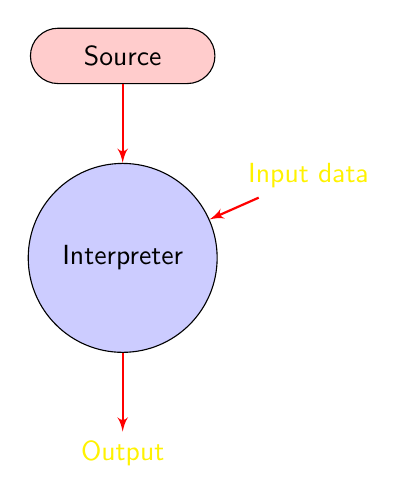
\begin{tikzpicture}[font=\sffamily,remember picture,
  block/.style = {circle, draw, fill=blue!20, text centered, text
    width=6em, rounded corners, minimum height=4em},
  cloud/.style = {rectangle, draw, fill=red!20, text centered, text
    width=6em, rounded corners=10pt, minimum height=2em},
  data/.style = {rectangle, draw=none, yellow, text centered},
  line/.style = {-latex', red, thick}]

  \node [cloud] (src) {Source};
  \node [block, below=of src] (int) {Interpreter};
  \node [data] (dat) at ([xshift=5em]int.60) {Input data};
  \node [data, below=of int] (out) {Output};

  \draw [line] (src) -- (int);
  \draw [line] (dat) -- (int);
  \draw [line] (int) -- (out);

\end{tikzpicture}
\end{document}
